\subsection{Person-disjoint cohort and repeated-cycle analysis}
\label{sec:cohort-cycle-results}

\paragraph{Coverage and model diagnostics.}
The audited A6 cross-fit contains all 137 participants and 928 eligible cycles:
539 from elderly-labeled and 389 from student-labeled participants. All eight
centered primary mixed models converged without a person-permutation fallback.
Six retained person-specific random intercepts and cycle-position slopes;
axial ROM and wrist wrapping used the prespecified random-intercept fallback
because their slope covariance was singular. Maximum standardized residuals and
variance components are archived with the generated results.

\begin{table}
\centering
\caption{Out-of-fold cohort and repeated-cycle analysis. Cohort effects are elderly-minus-student mixed-model coefficients at the mid-repetition reference (normalized cycle position 0.5); angular speed, duration, and repeatability use log models. MAD effects are person-level median differences. Values are estimated kinematic descriptors, not clinical joint angles.}
\label{tab:cohort_cycle_results}
\scriptsize
\resizebox{\linewidth}{!}{%
\begin{tabular}{lcccccc}
\toprule
Outcome & Elderly median [IQR] & Student median [IQR] & Cohort effect [95\% CI] & $p_{\mathrm{Holm}}$ & MAD effect ($p_{\mathrm{Holm}}$) & Cohort$\times$cycle ($p_{\mathrm{Holm}}$) \\
\midrule
Axial rotation ROM & 0.831 [0.750, 0.971] & 0.881 [0.696, 0.979] & 0.2475 [-0.0242, 0.5192] & 0.2966 & -0.0016 (1.0000) & -0.0837 (1.0000) \\
Angular speed (P95) & 2.033 [1.714, 3.021] & 1.904 [1.675, 2.198] & 0.3006 [0.1136, 0.4876] & 0.0114 & 0.0314 (0.4459) & -0.0363 (1.0000) \\
Peak rotation phase & 0.460 [0.430, 0.904] & 0.460 [0.440, 0.900] & -0.0013 [-0.0568, 0.0542] & 1.0000 & 0.0000 (1.0000) & 0.0156 (1.0000) \\
Trunk tilt (P95) & 0.040 [0.033, 0.049] & 0.036 [0.030, 0.045] & 0.0042 [0.0002, 0.0082] & 0.2514 & -0.0002 (1.0000) & -0.0005 (1.0000) \\
Wrist wrapping (P95) & 3.021 [2.502, 3.060] & 3.027 [2.442, 3.061] & 0.0289 [-0.0626, 0.1204] & 1.0000 & -0.0073 (1.0000) & -0.0115 (1.0000) \\
Cycle duration & 2.638 [2.625, 2.650] & 2.650 [2.633, 2.667] & -0.0127 [-0.0256, 0.0002] & 0.2677 & 0.0083 (1.0000) & -0.0127 (1.0000) \\
Log dimensionless jerk & 10.178 [10.019, 10.621] & 10.097 [9.970, 10.315] & 0.4233 [0.2336, 0.6130] & 0.0001 & 0.0377 (0.0208) & -0.0167 (1.0000) \\
Whole-body repeatability & 0.016 [0.014, 0.019] & 0.016 [0.013, 0.019] & -0.0145 [-0.1055, 0.0765] & 1.0000 & -0.0003 (1.0000) & 0.0347 (1.0000) \\
\bottomrule
\end{tabular}%
}
\end{table}


\paragraph{Mid-repetition cohort contrasts.}
At normalized cycle position 0.5, the elderly coefficient for
95th-percentile angular speed is 0.3006 on the log scale (95\% CI
0.1136--0.4876, $p_{\mathrm{Holm}}=0.0114$), corresponding to a ratio of
1.351 (95\% CI 1.120--1.628). Log dimensionless angular jerk is 0.4233
higher (95\% CI 0.2336--0.6130,
$p_{\mathrm{Holm}}<0.0001$). Axial ROM, peak phase, wrist wrapping, cycle
duration, and whole-body repeatability do not show corrected cohort differences.
Trunk tilt has an uncorrected $p=0.0419$ but does not survive correction
($p_{\mathrm{Holm}}=0.2514$).

Omitting the artificial outer-fold fixed effects yields closely matched
coefficients: 0.2972 for log angular speed
($p_{\mathrm{Holm}}=0.0186$) and 0.4161 for log jerk
($p_{\mathrm{Holm}}=0.0004$). This sensitivity shows that the two primary
contrasts are not created by the outer-fold indicators.

\paragraph{Within-person cycles and repetition order.}
Only log dimensionless jerk shows a corrected cohort difference in
within-person dispersion. The elderly-minus-student difference in person-level
MAD is 0.0377 (bootstrap 95\% CI 0.0135--0.0735,
$p_{\mathrm{Holm}}=0.0208$). None of the other seven MAD contrasts survives
correction. All eight cohort-by-cycle-position interactions have
$p_{\mathrm{Holm}}=1.000$. The data therefore provide no evidence for a
different monotonic first-to-last repetition trend between cohorts.

\begin{figure}
\centering
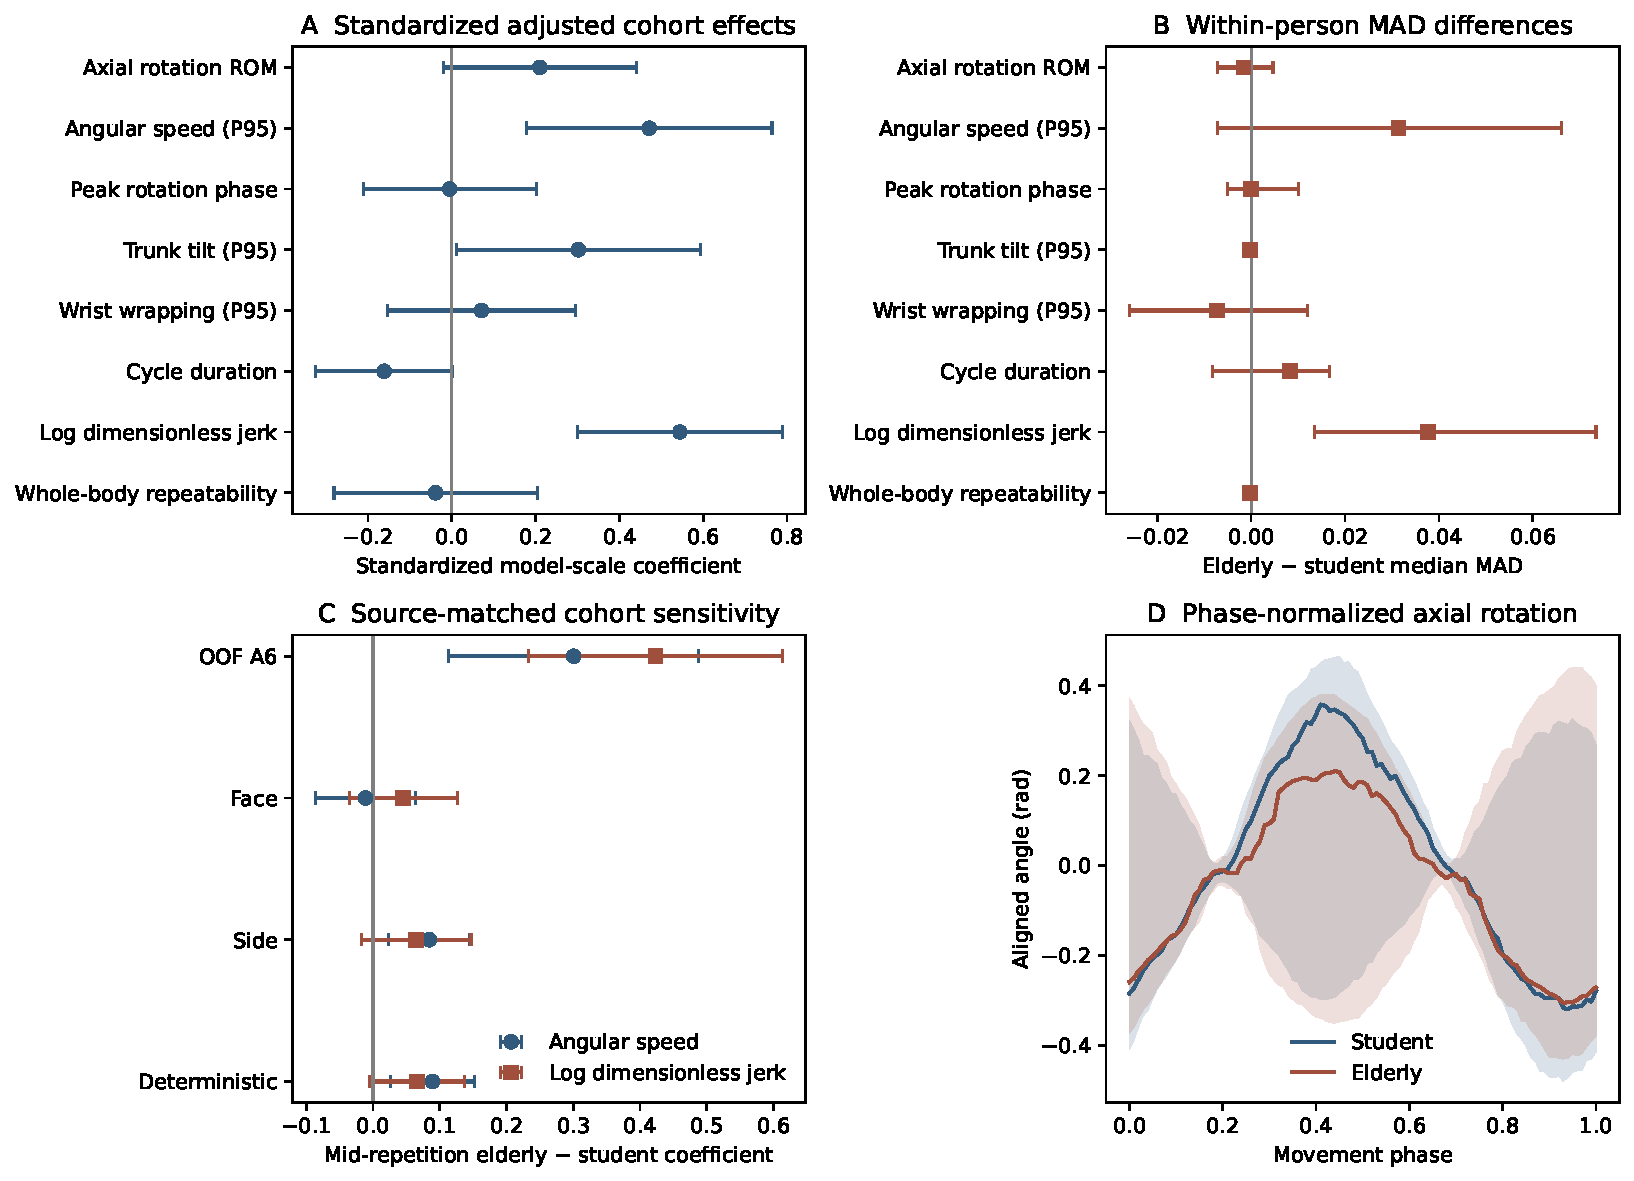
\includegraphics[width=\linewidth]{figures/cohort_cycle_analysis.pdf}
\caption{Person-disjoint cohort analysis. (A) Standardized mid-repetition
mixed-model cohort effects. (B) Person-level within-person MAD differences.
(C) Source-matched centered mixed-model sensitivity for angular speed and log
dimensionless jerk. Error bars are 95\% confidence intervals. (D)
Person-median phase-normalized axial rotation with interquartile bands; no
axial-angle cluster survives correction across descriptor families.}
\label{fig:cohort-cycle-analysis}
\end{figure}

\paragraph{Phase-localized comparisons.}
No axial-angle or angular-speed cluster is significant after across-descriptor
Holm correction. Trunk-tilt clusters remain at phases 0.19--0.36 and
0.73--0.87 (both adjusted $p=0.0040$) and 0.91--1.00
($p=0.0130$). Wrist wrapping differs over phase 0.30--0.57
($p=0.0237$). These secondary, model-derived localizations are
hypothesis-generating and not anatomical validation.

\begin{table*}[t]
\centering
\caption{Pose-source sensitivity using the same centered cycle-level mixed model
as the primary analysis. Cells report the mid-repetition
elderly-minus-student coefficient [95\% CI] with
$p_{\mathrm{Holm}}$ corrected across eight outcomes within each source.}
\label{tab:cohort-cycle-sensitivity}
\scriptsize
\resizebox{\linewidth}{!}{%
\begin{tabular}{l c c c c}
\toprule
Outcome & OOF A6 & Face only & Side only & Deterministic \\
\midrule
Angular speed (P95) & 0.3006 [0.1136, 0.4876] (0.0114) & -0.0111 [-0.0861, 0.0639] (1.0000) & 0.0843 [0.0233, 0.1452] (0.0337) & 0.0891 [0.0264, 0.1519] (0.0323) \\
Log dimensionless jerk & 0.4233 [0.2336, 0.6130] (0.0001) & 0.0452 [-0.0357, 0.1261] (1.0000) & 0.0646 [-0.0177, 0.1468] (0.2475) & 0.0657 [-0.0056, 0.1369] (0.2324) \\
\bottomrule
\end{tabular}%
}
\end{table*}


\paragraph{Pose-source sensitivity.}
Applying the same centered cycle-level model to each pose source materially
changes the magnitude. For log angular speed, the cohort coefficient is
0.3006 for OOF A6, $-0.0111$ for face, 0.0843 for side, and 0.0891 for
deterministic fusion; only A6, side, and deterministic fusion survive their
within-source Holm families. For log jerk, A6 is 0.4233, whereas face, side,
and deterministic estimates are 0.0452, 0.0646, and 0.0657 and none of the
latter is corrected-significant. The A6 application signals are therefore
pose-source-sensitive and may reflect learned representation effects as well as
movement differences.

As a separate participant-balanced estimand, person-median permutations do not
show corrected A6 differences for angular speed
($p_{\mathrm{Holm}}=0.8783$) or jerk
($p_{\mathrm{Holm}}=0.5159$). This estimand difference further limits the
cohort analysis to an exploratory application demonstration.
